\begin{titlepage}\centering
\vspace*{\fill}

\chapter{Adaptive continuation SIMP}\thispagestyle{EmptyHeader}
\label{chp:2}

\begin{tcolorbox}
This work appears in the paper: "Adaptive continuation solid isotropic material with penalization for volume constrained compliance minimization", Computer Methods in Applied Mechanics and Engineering, Volume 363, 2020. \citep{TAREK2020112880}
\end{tcolorbox}

\vspace*{\fill}
\end{titlepage}

\newpage

\section{Introduction}

The main drawback of CSIMP compared to the single penalty SIMP is that it usually requires a large number of FEA simulations to converge. This is in contrast to the BESO algorithm in the VCCM class of problems which was shown to converge in much fewer FEA simulations to an equally good solution by \cite{Huang2010a} when solving the cantilever and Messerschmitt-Bolkow-Blohm (MBB) beam VCCM problems, shown in Figures \ref{fig:CantBeam1} and \ref{fig:MBBBeam} respectively. In MMA, each iteration requires the evaluation of the objective's and constraints' zero and first order information, i.e. function values and gradients. Obtaining these requires solving a finite element analysis (FEA) simulation which in the VCCM case solves the system $\bm{K}\bm{u}=\bm{f}$. The time each FEA simulation takes grows significantly with the size of the ground mesh so reducing the number of such simulations is crucial to improve the scalability of CSIMP.

\begin{figure}
  \centering
  \resizebox{\textwidth}{!}{
    \begin{tikzpicture}
        \draw[fill,color=gray!70] (0,-0.1) rectangle (-0.3,2.1);
        \node [align=center, body,line width=1.2pt,minimum height=2cm,minimum width=8cm,anchor=south west] (body1) at (0,0) {};
        \draw (body1.south east) -- ++(1,0) coordinate (D1) -- +(5pt,0);
        \draw (body1.north east) -- ++(1,0) coordinate (D2) -- +(5pt,0);
        \draw [dimen] (D1) -- (D2) node {40mm};

        \draw (body1.north west) -- ++(0,0.5) coordinate (D1) -- +(0,5pt);
        \draw (body1.north east) -- ++(0,0.5) coordinate (D2) -- +(0,5pt);
        \draw [dimen] (D1) -- (D2) node {160mm};
        \draw[->,line width=1pt] (8,1) -- (8.15,1) -- (8.15,0.2);
        \node (arrowhead) at (8.4,0.25) {F};
    \end{tikzpicture} \newline
  }
  \caption{Cantilever beam problem before topology optimization.}
  \label{fig:CantBeam1}
\end{figure}

\begin{figure}
  \centering
  \begin{subfigure}{\textwidth}
    \resizebox{1\textwidth}{!}{
      \begin{tikzpicture}[>=latex]
        \draw[line width=1.2pt] (-6,0) rectangle (6,2);
          \draw (6,0) -- ++(0.7,0) coordinate (D1) -- +(5pt,0);
          \draw (6,2) -- ++(0.7,0) coordinate (D2) -- +(5pt,0);
          \draw [dimen] (D1) -- (D2) node {20mm};
          \draw (-6,2) -- ++(0,1.3) coordinate (D3) -- +(0,5pt);
          \draw (6,2) -- ++(0,1.3) coordinate (D4) -- +(0,5pt);
          \draw [dimen] (D3) -- (D4) node {120mm};

        \draw (-6,0) -- (-6.2,-0.3) -- (-5.8,-0.3) -- cycle;
        \draw (-6.15,-0.36) circle (0.06);
        \draw (-5.85,-0.36) circle (0.06);
        \node [marked body,minimum height=0.1cm,minimum width=1cm,anchor=center] at (-6,-0.42-0.05) {};

        \draw (6,0) -- (6.2,-0.3) -- (5.8,-0.3) -- cycle;
        \node [marked body,minimum height=0.1cm,minimum width=1cm,anchor=center] at (6,-0.35) {};

        \draw[->,line width=1pt] (0,3) -- (0,2);
        \node (arrowhead) at (0.2,2.7) {F};
      \end{tikzpicture}
    }
    \caption{Full beam}
    \label{fig:FullMBB}
  \end{subfigure}
  \begin{subfigure}{0.5\textwidth}
    \hfill
    \resizebox{1\textwidth}{!}{
      \begin{tikzpicture}[>=latex]
        \draw[line width=1.2pt] (0,0) rectangle (6,2);
        \draw (6,0) -- ++(0.7,0) coordinate (D1) -- +(5pt,0);
        \draw (6,2) -- ++(0.7,0) coordinate (D2) -- +(5pt,0);
        \draw [dimen] (D1) -- (D2) node {20mm};
        \draw (0,2) -- ++(0,0.5) coordinate (D3) -- +(0,5pt);
        \draw (6,2) -- ++(0,0.5) coordinate (D4) -- +(0,5pt);
        \draw [dimen] (D3) -- (D4) node {60mm};

        \draw (0,2) -- (-0.3,2.2) -- (-0.3,1.8) -- cycle;
        \draw (-0.36,2.15) circle (0.06);
        \draw (-0.36,1.85) circle (0.06);
        \node [marked body,minimum height=1cm,minimum width=0.1cm,anchor=center] at (-0.42-0.05,2) {};

        \draw (0,1) -- (-0.3,1.2) -- (-0.3,0.8) -- cycle;
        \draw (-0.36,1.15) circle (0.06);
        \draw (-0.36,0.85) circle (0.06);
        \node [marked body,minimum height=1cm,minimum width=0.1cm,anchor=center] at (-0.42-0.05,1) {};

        \draw (0,0) -- (-0.3,0.2) -- (-0.3,-0.2) -- cycle;
        \draw (-0.36,0.15) circle (0.06);
        \draw (-0.36,-0.15) circle (0.06);
        \node [marked body,minimum height=1cm,minimum width=0.1cm,anchor=center] at (-0.42-0.05,0) {};
        
        \draw (6,0) -- (6.2,-0.3) -- (5.8,-0.3) -- cycle;
        \draw (6.15,-0.36) circle (0.06);
        \draw (5.85,-0.36) circle (0.06);
        \node [marked body,minimum height=0.1cm,minimum width=1cm,anchor=center] at (6,-0.42-0.05) {};

        \draw[->,line width=1pt] (0,3) -- (0,2);
        \node (arrowhead) at (0,3.2) {F};
      \end{tikzpicture}
    }
    \caption{Half beam}
    \label{fig:HalfMBB}
  \end{subfigure}
  \caption{Messerschmitt-Bolkow-Blohm (MBB) beam problem}
  \label{fig:MBBBeam}
\end{figure}


In the rest of this chapter, the compliance will be defined as:
  \begin{align} \label{eqn:compliance}
    & C = \bm{u}^T\bm{K}\bm{u} = \bm{f}^T\bm{K}^{-1}\bm{f} 
  \end{align}
i.e. twice the strain energy of the system, where $\bm{K}$ is the stiffness matrix assembled from element stiffness matrices, $\bm{u}$ is the displacement vector of all the degrees of freedom of the ground mesh, such that $u_i$ corresponds to the $i^{th}$ degree of freedom of the ground mesh, and $\bm{f}$ is the load vector assembled from surface and point loads. The relationship between the global and element stiffness matrices is given by:
  \begin{gather} \label{eqn:assembly}
    \bm{K} = \sum\limits_e \rho_e(P(x_e)) \bm{K}_e \\
    \rho_e(x_e) = (1-x_{min})x_e + x_{min}
  \end{gather}
where $\bm{K}_e$ is the element stiffness matrix of element $e$, which describes the relationship between the degrees of freedom inside element $e$, and such that the $(i,j)$th entry of $\bm{K}_e$ is 0 if either degree of freedom $i$ or $j$ is not in element $e$, $P$ is the penalty function with a penalty value $p$, and $x_{min}$ is chosen to be a small value, e.g. 1e-3, to stop $\bm{K}$ from becoming singular when a node is not part of any solid element.

\section{Literature review}

Some efforts can be found in literature towards decreasing the computational burden of continuation SIMP and topology optimization at large. For instance, approximate reanalysis via reusing the stiffness matrix decomposition in direct linear solvers was proposed by Amir et al. \cite{Amir2009}. Later, approximate analysis via reusing the preconditioner in the preconditioned conjugate gradient (PCG) algorithm was also successfully applied to solve compliance problems \citep{Amir2015}. The decomposition reuse approach was then extended to approximately solve the eigenvalue problem found in topology optimization of oscillating systems \citep{Zheng2017}. Use of multi-resolution meshes and adaptive mesh refinement can also be found in topology optimization literature. For instance, Amir et al. \cite{Amir2014} used a geometric multigrid preconditioner in the PCG algorithm based on a multi-resolution mesh. Adaptive mesh refinement can also be found in numerous old and recent works, e.g. \cite{Maute1995,Maute1997,Stainko2006,Wang2010a,Wang2010a,Bruggi2011,Wang2013,Wang2014,SalazardeTroya2018,Lambe2018}.

A few works also studied some penalty adaptation routines. \cite{Dadalau2009} provided a way to adapt the penalty step which was used along with a variant of the optimality criteria method for VCCM problems. More specifically, \cite{Dadalau2009} set the penalty in each iteration such that it maximizes the ratio of the standard deviation of elements' fractional volumes, $\sigma(v_e x_e)$, and the strain energy, i.e. half the compliance. Maximizing this ratio is supposed to maximize the closeness to a binary solution, without compromising the compliance too much. However, there are two questionable points in this approach, beside not having a proof. Firstly, the standard deviation of elements' fractional volumes is not an accurate measure of how binary a solution is; it is a measure of spread around the mean. This means that the direction in which the standard deviation increases for any one element is always away from the mean. For instance, let the volume of each element be $1.0$, and let all elements have $x_e = 0.3 \quad \forall e$, therefore the mean is $0.3$ and standard deviation is $0$. Making one $x_e = 0.5$, i.e. clearly more fractional, will increase the standard deviation to a strictly positive value, thus falsely claiming that the new solution is closer to a 0-1 design. When the volume constraint is active, the mean value of $x_e$, weighted by the element volumes, is exactly the volume fraction. The second problem with the approach proposed by \cite{Dadalau2009} is that as shown in their experiments, the penalty value $p$ is allowed to freely increase or decrease with no control over the final penalty, which means that SIMP's (or RAMP's) property of converging to a binary solution for VCCM problems with a high penalty is lost.

Another penalty adaptation approach was proposed by \cite{GaoXingjun2017} for buckling constrained compliance minimization problems. \cite{GaoXingjun2017} chose the penalty in each subproblem to promote a certain amount of constraint violation such that the eigenvalue constraint is violated by 0.1 if possible while maintaining an increasing penalty. This was motivated by the observation that for low penalty values, all the buckling load factors are typically over the threshold, so the stability constraint is not active and does not contribute to the optimization process. However, when the penalty increases, the violated stability constraints require a re-distribution of the material, which when the problem is non-convex, may converge to a bad and/or infeasible solution. The heuristic proposed was shown to improve the stability of the solution, though still infeasible, at the expense of a higher compliance.

However most notably, \cite{Rojas-Labanda2015} tried to reduce the number of FEA simulations needed by CSIMP for generic topology optimization problems using a number of alternative approaches, the most significant of which was the \textit{automatic} continuation SIMP (Auto-CSIMP). In auto-CSIMP the penalty $p$ is treated as a variable and a constraint is defined such that it is feasible only when $p = p_{max}$. A nonlinear equality (or inequality) constraint $g(p;\mu) = 0$ (or $\leq 0$) is added, where $\mu$ is a hyperparameter, and the whole problem is solved using a first order NLP solver which solves for $p$ and $\bm{x}$ simultaneously, using linear approximation of the nonlinear constraints, such as the interior point optimizer IPOPT \citep{Wachter2006}. The main purpose of this additional constraint is to stall the convergence of the algorithm achieving a similar effect as the original CSIMP. While this method was shown to successfully decrease the number of simulations needed to converge, there are a few questionable points about the algorithm. Firstly, the choice of $g(p;\mu)$ and its hyperparameter $\mu$ seem largely arbitrary with the exception of being a decreasing function in $p$ which was derived from Newton's method applied on the KKT conditions of the barrier problem used in IPOPT. However, the analysis of the number of iterations needed to reach the final penalty for different functions $g$ and values of $\mu$ is not accurate since it assumes a fixed step size of $\alpha = 1$ in Newton's method. So it is not clear that the choice of $g(p;\mu)$ or its hyperparameter thereof will never result in IPOPT satisfying the penalty constraint too quickly thus approaching the behavior of a single penalty SIMP. In the paper by \cite{Wachter2006} which describes the algorithm used in IPOPT, the actual step $\alpha_k$ is influenced by the search direction in $[\bm{x}; p]$, which is a function of: 
  \begin{enumerate}[label=(\arabic*)]
    \item the Hessian of the Lagrangian of the barrier problem with respect to $[\bm{x}; p]$, 
    \item the Jacobian of the constraints with respect to $[\bm{x}; p]$, and 
    \item the initial primal and dual solutions. 
  \end{enumerate}
  Moreover, $\alpha_k$ is ultimately determined by how the objective and constraints change along the search direction during the backtracking line search for [$\bm{x}; p]$ combined, as well as the line search's stopping criteria. Additionally, the search direction can itself be influenced by the step size in case the second order correction step is performed. The influence of factors like the number of elements, the volume of each element, the Young's modulus and Poisson's ratio of the material on the step size that IPOPT takes was not studied and is indeed difficult to measure; so the risk of premature convergence of the penalty constraint exists. Secondly, it seems unclear whether using a different NLP solver or improving the existing IPOPT solver will result in a better or worse Auto-CSIMP. While Auto-CSIMP is, in theory, possible to use for any topology optimization problem and was shown to outperform the traditional MMA-based CSIMP with a large penalty step by \cite{Rojas-Labanda2015}, the design space for MMA-based CSIMP algorithms has not been fully explored yet.

\section{Penalty adaptation} \label{sec:adaptive_penalty}

  In every CSIMP subproblem, an NLP is solved using a certain penalty value $p$ until convergence before moving on to the next penalty value. When using the KKT stopping criteria, at every penalty step, there is at least 1 FEA simulation to be performed in order to check for convergence. However in certain phases of CSIMP, e.g. near convergence, changing the value of $p$ is not likely to change the solution or the objective much. Therefore, one improvement that can be employed is to use the last solution $\bm{u}$ from the last FEA simulation of the previous subproblem with the new penalty value to estimate the change in the objective value. If the change is large enough, the subproblem can be solved, otherwise, the penalty can be incremented right away saving unnecessary FEA simulations. The new subproblem's tolerance can be used as this criteria. This provides a simple way to adapt the penalty step not to perform unnecessary FEA simulations. 

  To develop some mathematical intuition for this approach, let's assume the relative change in the objective stopping criteria is used for the MMA, together with solution feasibility. One can then attempt to estimate the effect of $p$ on the optimal value $C^*$, through a first order Taylor series expansion of $C^*(p)$, which is the optimal value of $C$ for each penalty value $p$. Assuming that the local optimal solution $\bm{x}^*$ is a KKT point of the subproblem at the current $p$ and that the optimal primal-dual solution, the objective and constraints are continuous and differentiable functions of $p$, it is possible to prove that:
  \begin{align} \label{eqn:fullderivative}
    & \frac{dC^*(p)}{dp} = \frac{\partial C}{\partial p} - \sum_i{\lambda_i \frac{\partial h_i}{\partial p}}
  \end{align}
  where $h_i$ is the $i^{th}$ constraint, and $\lambda_i$ is the corresponding Lagrangian multiplier. For the VCCM problem, this is simply $\frac{dC^*(p)}{dp} = \frac{\partial C}{\partial p}$ since the constraints are not a function of $p$. This also means that the value of $p$ does not change the feasibility status of a solution.

  \begin{proof}
    Let $\bm{x}(p)$ now denote the optimal solution $\bm{x}^*$ given a certain value of $p$. The KKT conditions guarantee that:
    \begin{align} \label{eqn:kkt1}
      & -\nabla_{\bm{x}} C + \sum_i \lambda_i \nabla_{\bm{x}} h_i = \bm{0}
    \end{align}
    The full derivative of the optimal compliance $C^*(p) = C(\bm{x}(p), p)$ with respect to $p$ is:
    \begin{align}
      & \frac{dC^*(p)}{dp} = \frac{\partial C(p)}{\partial p} + \nabla_{\bm{x}} C \cdot \frac{d\bm{x}(p)}{dp}
    \end{align}
    Taking the dot product of the LHS and RHS of equation \ref{eqn:kkt1} with $\frac{d\bm{x}(p)}{dp}$ and adding $-\frac{\partial C}{\partial p}  + \sum_i \lambda_i \frac{\partial h_i}{\partial p}$ to both sides, one can show that:
    \begin{align} \label{eqn:presimpl_fullderivative}
      & -\frac{dC^*}{dp} + \sum_i \lambda_i \frac{dh^*_i}{dp} = -\frac{\partial C}{\partial p}  + \sum_i \lambda_i \frac{\partial h_i}{\partial p}
    \end{align}
    where $h^*_i = h_i(\bm{x}(p), p)$.
    Furthermore, the complementarity slackness property of the KKT solution specifies that:
    \begin{align} \label{eqn:compl_slackness}
      & \lambda_i(p) h_i(\bm{x}(p), p) = 0
    \end{align}
    Using the product rule:
    \begin{align}
      & \frac{d\lambda_i(p)}{dp} h_i(\bm{x}(p), p) + \lambda_i(p) \frac{d h_i(\bm{x}(p), p)}{dp} = 0
    \end{align}
    Multiplying both sides by $\lambda_i(p)$ and using equation \ref{eqn:compl_slackness}, one can show that:
    \begin{align}
      & \lambda_i(p)^2 \frac{d h_i(\bm{x}(p), p)}{dp} = 0
    \end{align}
    so either $\lambda_i(p) = 0$ or $\frac{d h_i(\bm{x}(p), p)}{dp} = 0$. In other words, equation \ref{eqn:presimpl_fullderivative} simplifies into equation \ref{eqn:fullderivative}. \textit{This completes the proof}.
  \end{proof}

  Let $\bm{u}$, $\bm{x}$ and $p$ be independent variables, as in Simultaneous Analysis and Design (SAND). The partial derivative of $C$ with respect to $p$ is:
  \begin{align}
    & \frac{\partial{C(\bm{u}, \bm{x}, p)}}{\partial{p}} = \bm{u}^T \frac{\partial \bm{K}(\bm{x}, p)}{\partial p} \bm{u} \\
    & \frac{\partial \bm{K}(\bm{x}, p)}{\partial p} = \sum\limits_e log(x_e) \times x_e^p \times \bm{K}_e
  \end{align}
  Note that this function is discontinuous at any point where some $x_e = 0$. However, using L'Hopital's rule on $\frac{log(x_e)}{1/x_e^p}$, $\lim_{x_e \to 0} log(x_e) \times x_e^p = -\frac{x_e^p}{p} = 0$. Therefore, $\frac{\partial \bm{K}}{\partial p}$ can be numerically defined as:
  \begin{align}
    \frac{\partial \bm{K}}{\partial p} = \sum\limits_e \Gamma_e \times \bm{K}_e \\ 
    \Gamma_e = \begin{cases}
      log(x_e) \times x_e^p & x_e \geq \epsilon \\
      0 & x_e < \epsilon
    \end{cases}
  \end{align}
  for some small $\epsilon$. 

  Incidentally, $\frac{\partial{C(\bm{u}, \bm{x}, p)}}{\partial{p}}$, when $\bm{u}$ is treated as a variable, is equal to $-\frac{\partial C(\bm{x}, p)}{\partial p}$ when treating $\bm{u}$ as a function of $\bm{x}$ and $p$, as in Nested Analysis and Design (NAND). Since $\bm{u}(\bm{x}, p)$ is implicitly defined by:
  \begin{align}
    & \bm{K}(\bm{x}, p) \bm{u}(\bm{x}, p) = \bm{f}
  \end{align}
  then:
  \begin{align}
    & \frac{\partial \bm{K}}{\partial p} \bm{u} + \bm{K} \frac{\partial \bm{u}}{\partial p} = 0 \nonumber \\
    & \frac{\partial \bm{u}}{\partial p} = -\bm{K}^{-1} \frac{\partial \bm{K}}{\partial p} \bm{u}
  \end{align}
  Hence, the partial derivative of $C(\bm{x}, p) = \bm{u}(\bm{x}, p)^T \bm{K}(\bm{x}, p) \bm{u}(\bm{x}, p)$ with respect to $p$ is:
  \begin{align}
    \label{eqn:partialCpartialp}
    \frac{\partial C(\bm{x}, p)}{\partial p} & = 2 \bm{u}^T \bm{K} \frac{\partial \bm{u}}{\partial p} + \bm{u}^T \frac{\partial \bm{K}}{\partial p} \bm{u} \nonumber \\
    & = -\bm{u}^T \frac{\partial \bm{K}}{\partial p} \bm{u}
  \end{align}
  Since $x_e \leq 1$, and $\bm{K}_e$ is positive semi-definite for all $e$, the above term is non-negative. In this chapter, the NAND framework is used.

  Assuming the first order approximation, it is also possible to choose the penalty step $\Delta p_k$ such that the approximate compliance:
  \begin{align}
    \tilde{C}_{k} = C(\bm{u}_{k-1}, \bm{x}_{k-1}, p_{k-1} + \Delta p_k) \approx C_{k-1} + \frac{\partial C}{\partial p}(\bm{u}_{k-1}, \bm{x}_{k-1}, p_{k-1}) \times \Delta p_k
  \end{align}
  satisfies inequality (\ref{eqn:tolerance})\begin{align}
    \label{eqn:tolerance}
    |C_{k-1} - C_{k}| / |C_{k-1}| < tol 
  \end{align}
  for some tolerance  $tol$. Choosing $\Delta p$ such that:
  \begin{align}
    |C_{k-1} - \tilde{C}_{k}| / |C_{k-1}| = \beta \times tol
  \end{align}
  for some $\beta \geq 1$, we get:
  \begin{align}
    \label{eqn:blind_adaptive_step}
    \Biggl| \frac{\partial C}{\partial p}\Biggr| \frac{\Delta p}{|C_{k-1}|} = \beta \times tol \nonumber \\
    \Delta p = \frac{\beta \times tol \times |C_{k-1}|}{| \partial C / \partial p|}
  \end{align}

  On the other hand, using blind penalty adaptation with $\Delta p = \Delta p_0 \times n$ for $n \in \mathbb{N}$, where $\Delta p_0$ is the fixed step in CSIMP, the benefit of penalty adaptation can only be observed when $n > 1$, that is some subproblem is skipped because it is deemed unnecessary. The condition for $n > 1$ is:
  \begin{align}
    \Delta p_0 \leq \frac{tol \times |C_{k-1}|}{|\partial C / \partial p|}    
  \end{align}
  More generally, the condition for $i$ subproblems to be skipped, i.e. $\Delta p \geq \Delta p_0 \times (i + 1)$ is:
  \begin{align}
    \Delta p_0 \times i \leq \frac{tol \times |C_{k-1}|}{| \partial C / \partial p|}    
  \end{align}
  Not surprisingly, the penalty adaptation trick can be observed to be more effective in skipping subproblems for small $\Delta p_0$ and large $tol$. While the intuition above was developed using the relative change in objective value, computational experiments show a significant reduction in the number of FEA simulations from skipping subproblems when using the more rigorous KKT stopping criteria.

\section{Test Problems} \label{sec:test_problems}

  \begin{figure}
  \centering
  \resizebox{\textwidth}{!}{
    \begin{tikzpicture}[>=latex]
        \draw[fill,color=gray!70] (-0.2,2) rectangle (3.2,2.5);
        \draw[line width=1.2pt] (0, 2) node(nodeA){} -- (3, 2) node(nodeB){} -- (3, -1) -- (6, -1) node(nodeC){} -- (6, -4) node(nodeD){} -- (0, -4) node(nodeE){} -- cycle;
        
        \draw (nodeA) -- ++(0,1) coordinate (D1) -- +(0,5pt);
        \draw (nodeB) -- ++(0,1) coordinate (D2) -- +(0,5pt);
        \draw [dimen] (D1) -- (D2) node {50 mm};

        \draw (nodeA) -- ++(-1,0) coordinate (D1) -- +(-5pt,0);
        \draw (nodeE) -- ++(-1,0) coordinate (D2) -- +(-5pt,0);
        \draw [dimen] (D1) -- (D2) node {100 mm};

        \draw (nodeC) -- ++(1,0) coordinate (D1) -- +(5pt,0);
        \draw (nodeD) -- ++(1,0) coordinate (D2) -- +(5pt,0);
        \draw [dimen] (D1) -- (D2) node {50 mm};

        \draw (nodeE) -- ++(0,-1) coordinate (D1) -- +(0,-5pt);
        \draw (nodeD) -- ++(0,-1) coordinate (D2) -- +(0,-5pt);
        \draw [dimen] (D1) -- (D2) node {100 mm};

        \draw[->,line width=1pt] (6,-2.5) -- (6.2,-2.5) -- (6.2,-3.15);
        \node (arrowhead) at (6.2,-3.25) {F};
    \end{tikzpicture} \newline
  }
  \caption{L-shaped beam problem}
  \label{fig:LBeam}
\end{figure}


  There is a wide array of test problems used in literature to evaluate topology optimization algorithms. In the majority of papers, a few test problems are used to demonstrate the effect of algorithms, e.g. \cite{Huang2010a}, \cite{Stolpe2001a}, and \cite{SalazardeTroya2018}. \cite{Valdez2017} compiled a list of linearly elastic 2D structures commonly used as test problems in literature. Another set of problems for compliant mechanisms was also proposed by \cite{Deepak2009}. However, perhaps the largest set of benchmark problems ever used in literature was by \cite{Rojas-Labanda2015a, Rojas-Labanda2015}. Rojas-Labanda et al. used a library of 225 minimum compliance problems, 135 minimum volume and 150 compliant mechanism design problems in \cite{Rojas-Labanda2015a}. The same authors seem to have used a subset of this library in \cite{Rojas-Labanda2015}. In this chapter, three 2D VCCM problems, shown in Figures \ref{fig:CantBeam1}-\ref{fig:LBeam}, and 1 3D VCCM problem are used to highlight the effect of penalty adaptation. A possible future work is to perform a more extensive study on a larger library of problems.
  
  The first test problem is the 2D cantilever beam problem, Figure \ref{fig:CantBeam1}, which was solved by \cite{Huang2010a} to benchmark soft-kill BESO against CSIMP. The second test problem is the MBB problem, Figure \ref{fig:MBBBeam}, was solved in the classical paper by \cite{Sigmund2001}. Due to the symmetry of the problem, the problem in Fig. \ref{fig:FullMBB} is typically reduced to the problem in \ref{fig:HalfMBB} to reduce the area of the topology to be optimized. The third test problem is the L-beam problem, Figure \ref{fig:LBeam}, which was taken from the book by \cite{Bendsoe2004}. These three problems are all part of the 2D collection made by \cite{Valdez2017}. Finally, a 3D cantilever beam variant of the first test problem will be tested with a ground mesh of dimensions $60 \times 20 \times 20$.

  In the 2D test problems, a ground mesh of plane stress quadrilateral elements is used, where each element is a square of side length $1\text{mm}$, and a sheet thickness of $1 \text{mm}$. In the 3D cantilever beam problem, hexahedral elements are used, where each element is a cube of side length $1\text{mm}$. Linear isoparameteric interpolation functions are used in the MBB, L-beam and 3D cantilever beam problems, and quadratic isoparameteric interpolation functions are used in the 2D cantilever beam problem. The 2D cantilever beam problem with a low volume fraction and linear interpolation functions was found to produce some extremely ill-conditioned geometries with corner contacts, hence the use of quadratic interpolation functions to achieve better accuracy in the FEA simulations. A Young's modulus of 1 MPa and Poisson's ratio of 0.3 are used in all the problems. A chequerboard density filter was used with a radius of 2 mm. The weights were calculated using the method described by \cite{Huang2010a}.

\section{Implementation} \label{sec:implementation}

  \subsection{Finite element analysis}

  All the topology optimization algorithms described in this chapter were implemented using the Julia programming language \citep{Bezanson2014} for handling generic unstructured, isoparameteric meshes. Finite element analysis was done with the help of the finite element tooling package JuAFEM.jl \footnote{https://github.com/KristofferC/JuAFEM.jl}. A direct Cholesky factorization based linear system solver for sparse matrices was used from SuiteSparse \footnote{http://faculty.cse.tamu.edu/davis/suitesparse.html} wrapped in Julia. The value of $x_{min}$ used was $0.001$ for all problems and algorithms since this is the standard value used in literature.

  \subsection{Optimization}

  The original MMA algorithm by \cite{Svanberg1987} was implemented and used to solve the SIMP subproblems. MMA parameters of $s_{init} = 0.5$, $s_{incr} = 1.2$ and $s_{decr} = 0.7$ were used as defined in the paper by \cite{Svanberg1987}. The dual problem of the convex approximation was solved using a log-barrier box-constrained nonlinear optimization solver, where the barrier problem was solved using the nonlinear CG algorithm for unconstrained nonlinear optimization \citep{Nocedal2006} as implemented in Optim.jl \footnote{https://github.com/JuliaNLSolvers/Optim.jl} \citep{KMogensen2018}. The nonlinear CG itself used the line search algorithm from Hager et al. \cite{Hager2006} as implemented in LineSearches.jl \footnote{https://github.com/JuliaNLSolvers/LineSearches.jl}.

  The stopping criteria used was similar to the one adopted by the KKT solver, IPOPT \citep{Wachter2006}. This stopping criteria is less scale sensitive than the KKT residual as it scales down the residual by a value proportional to the mean absolute value of the Lagrangian multipliers. Let the optimization problem be:
      \begin{mini!}|l|[3]
        {\bm{x}}{f(\bm{x})}{}{}
        \addConstraint {\quad \bm{c}(\bm{x}) \leq \bm{0}}{}
        \addConstraint {\quad 0 \leq x_e \leq 1}{\quad \forall e}
      \end{mini!}
  Let $\bm{\lambda}$ be the vector of Lagrangian multipliers of the nonlinear constraints, $\bm{z}_-$ be the vector of Lagrangian multipliers of the $\geq$ bound constraints, and $\bm{z}_+$ be the vector of Lagrangian multipliers of the $\leq$ bound constraints. The termination criteria used was:
    \begin{align}
      \max\Biggl\{\frac{||\nabla f(\bm{x}) + \nabla \bm{c}(\bm{x}) \bm{\lambda} + (\bm{z_+} - \bm{z_-})||_\infty}{s_d}, ||\bm{c}(\bm{x})_+||_\infty \Biggr\} \leq tol \\
      s_d = \max\Biggl\{s_{max}, \frac{||\bm{\lambda}||_1 + ||\bm{z_+} + \bm{z_-}||_1}{m + n} \Biggr\} / s_{max}
    \end{align}
  where $\bm{c}_+$ is the element-wise maximum of $\bm{c}$ and 0, and $s_{max}$ is a constant parameter. A value of $s_{max} = 100$ was used by \cite{Wachter2006} and the same is done in this work.

\section{Evaluating SIMP} \label{sec:evaluating_simp}

  There are a number of difficulties that one faces when trying to fairly assess the performance of SIMP variants to solve the VCCM problem:
  \begin{enumerate}
    \item The solution generated by SIMP is a continuous one, where $x_e$ is allowed to take fractional values. Therefore, the objective value is that of the continuous approximation of the problem. Moreover, $x_{min}$ and $P$ can affect the objective value differently for different ground mesh geometries.
    \item Obtaining a discrete solution from a continuous one can be done in different ways:
      \begin{enumerate}
        \item The solution can be rounded. This approach carries the risk of obtaining an infeasible solution after rounding even if the continuous solution was feasible.
        \item A projection function such as the regularized Heaviside projection function $f(x) = 1 - e^{\beta x} + x e^{-\beta}$ \citep{Guest2004} can be used to make the projected solution closer to a binary one. This method has the disadvantage of increasing the non-convexity of the optimization problem, requiring more iterations to converge, for $\beta > 0$. The regularized Heaviside function is the identity function when $\beta = 0$, and it gradually approximates the Heaviside step function as $\beta \to \infty$. A continuation over $\beta$ is therefore typically used. From experiments, using a high value of $\beta$ can cause numerical difficulties for the NLP solver because the slope at $x \approx 0$ becomes very high. Moreover, a very high value of $\beta$ is often required to get a near-binary solution.
        \item A subset of the elements can be selected based on their sorted $x_e$ values. In VCCM problems, this can be done by selecting the top $100V\%$ of the elements by $x_e$. However, for other constraints which require solving an FEA simulation to evaluate the feasibility of a solution, this approach is not straight forward to generalize. For constraints which are known to be satisfied with a full grid design, a bisection search can be used, adding or removing elements until a feasible binary solution is obtained.
      \end{enumerate}
      For the sake of this chapter, the regularized Heaviside projection was used together with the element selection method, where the top $100V\%$ elements were selected as per the projected filtered densities, then the discrete objective value was computed.
    \item After obtaining a discrete solution, the solution can exhibit chequerboard patterns, disconnected or undesired thin features. These are mostly visual features for which no metric in topology optimization literature exists as far as we know.
    \item Some SIMP variants can converge quickly to a solution with a good continuous objective value but a bad or undefined discrete objective value, due to disconnectivity or ill-conditioned geometries, e.g. corner contacts. For example in the VCCM problem, using a single low penalty value can generally lead to a lower continuous objective value, closer the lower bound which is the optimal value at $p = 1$, but the discrete design's objective value can be either infeasible or suboptimal.
  \end{enumerate}
  In SIMP literature, algorithms seem to be compared using their continuous objective values. Therefore, we do the same in this chapter. However, an additional metric will be added to measure how fractional a solution is. A more fractional solution is arguably a less trusted one since the continuous and discrete objectives are likely to be far apart. The measure of how fractional a solution is to be used in this chapter will be:
  \begin{align}
    \% frac = \frac{2 \sum\limits_e \min(x_e, 1 - x_e) \times v_e}{\sum\limits_e v_e} \times 100 \%
  \end{align}
  which is $0\%$ when a solution is fully binary, $100\%$ when a solution is all $0.5$ and it weighs the fractional part of a variable by the volume of the corresponding element. The fractionness of the solution will be evaluated using the projected filtered densities.
 
  In the following section, $\text{C-Obj}$ will refer to the objective value of the continuous optimal solution. This includes the effect of $x_{min}$, the density filter and projection. One additional metric to be used is the discrete design's objective value ($\text{D-Obj}$) after selecting the top $100V\%$ of the elements by their projected and filtered densities, and removing the void elements completely.

\section{Results and Discussion} \label{sec:penalty_adaptation_results}

  \subsection{Fixed tolerance}

  \begin{table}[H]
\centering
\tabcolsep=0.09cm
% table caption is above the table
\caption{The problem type and parameter settings of the experiments with continuation SIMP with a fixed tolerance.}
\label{tab:exp_params}
\begin{tabular}{|l|l|l|l|l||l|l|l|l|l|}
\hline\noalign{\smallskip}
Exp & Problem & $V$ & $tol$ & $\Delta p_0$ & Exp & Problem & $V$ & $tol$ & $\Delta p_0$ \\
\hline
1 & \multirow{ 8 }{*}{CantBeam} & \multirow{ 4 }{*}{0.3} & \multirow{ 2 }{*}{0.01} & 0.1 & 17 & \multirow{ 8 }{*}{LBeam} & \multirow{ 4 }{*}{0.3} & \multirow{ 2 }{*}{0.01} & 0.1\\
2 & & & & 0.05 & 18 & & & & 0.05\\
3 & & & \multirow{ 2 }{*}{0.0001} & 0.1 & 19 & & & \multirow{ 2 }{*}{0.0001} & 0.1 \\
4 & & & & 0.05 & 20 & & & & 0.05 \\
5 & & \multirow{ 4 }{*}{0.5} & \multirow{ 2 }{*}{0.01} & 0.1 & 21 & & \multirow{ 4 }{*}{0.5} & \multirow{ 2 }{*}{0.01} & 0.1 \\
6 & & & & 0.05 & 22 & & & & 0.05 \\
7 & & & \multirow{ 2 }{*}{0.0001} & 0.1 & 23 & & & \multirow{ 2 }{*}{0.0001} & 0.1 \\
8 & & & & 0.05 & 24 & & & & 0.05 \\
\hline
9 & \multirow{ 8 }{*}{HalfMBB} & \multirow{ 4 }{*}{0.3} & \multirow{ 2 }{*}{0.01} & 0.1 & 25 & \multirow{ 8 }{*}{3D CantBeam} & \multirow{ 4 }{*}{0.3} & \multirow{ 2 }{*}{0.01} & 0.1 \\
10 & & & & 0.05 & 26 & & & & 0.05 \\
11 & & & \multirow{ 2 }{*}{0.0001} & 0.1 & 27 & & & \multirow{ 2 }{*}{0.0001} & 0.1 \\
12 & & & & 0.05 & 28 & & & & 0.05 \\
13 & & \multirow{ 4 }{*}{0.5} & \multirow{ 2 }{*}{0.01} & 0.1 & 29 & & \multirow{ 4 }{*}{0.5} & \multirow{ 2 }{*}{0.01} & 0.1 \\
14 & & & & 0.05 & 30 & & & & 0.05 \\
15 & & & \multirow{ 2 }{*}{0.0001} & 0.1 & 31 & & & \multirow{ 2 }{*}{0.0001} & 0.1 \\
16 & & & & 0.05 & 32 & & & & 0.05 \\
\noalign{\smallskip}\hline
\end{tabular}
\end{table}

  \begin{table}
\centering
\tabcolsep=0.09cm
% table caption is above the table
\caption{This table shows the effect of penalty adaptation on CSIMP. The table shows the results of the experiments studying the effect of solution reuse on: 1) the number of FEA simulations (Sims) required by CSIMP, 2) the final objective of the continuous NLP at $p = 5$ (C-Obj), 3) the objective value of the rounded discrete solution (D-Obj), and 4) the percentage of fractionness (\% frac). The parameters of each experiment are described in Table \ref{tab:exp_params}}
\label{tab:csimp_reuse}
\begin{tabular}{|l|l|l|l|l||l|l|}
\hline\noalign{\smallskip}
Exp & \multicolumn{3}{c||}{\textbf{Fixed $\Delta p = \Delta p_0$}} & \multicolumn{3}{c|}{\textbf{\% Increase due to $\Delta p$ adaptation}}\\
\noalign{\smallskip}\hline\noalign{\smallskip}
& \textbf{Sims} & \textbf{C-Obj / D-Obj} & \textbf{\% frac} & \textbf{Sims} & \textbf{C-Obj / D-Obj} & \textbf{\% frac} \\
\hline
1 & 149 & 813.0/555.8 & 17.3 & -20.8 & -9.3/1.0 & -13.3 \\ 
\hline
2 &  213 & 742.2/572.4 & 14.3 & -45.1 & 1.6/-1.4 & 5.6 \\ 
\hline
3 &  291 & 720.4/549.2 & 14.1 & -18.2 & 0.5/-0.7 & 0.7 \\ 
\hline
4 &  485 & 712.5/559.9 & 13.8 & -18.1 & -0.3/0.5 & -0.7 \\ 
\hline
5 & 103 & 383.8/343.1 & 14.0 & -32.0 & -1.9/0.6 & -7.9 \\ 
\hline
6 & 149 & 382.7/338.3 & 12.4 & -53.0 & -0.1/1.7 & 6.5 \\ 
\hline
7 & 251 & 366.7/338.4 & 10.0 & -21.5 & 0.1/0.0 & 1.0 \\ 
\hline
8 & 376 & 366.9/338.0 & 9.9 & -24.5 & -0.0/0.2 & 0.0 \\ 
\hline
\hline
9 & 110 & 584.2/293.5 & 24.5 & -40.0 & 5.1/-0.4 & 2.0 \\ 
\hline
10 & 166 & 572.7/293.3 & 24.4 & -59.6 & 9.5/-0.3 & 2.9 \\ 
\hline
11 & 206 & 609.9/291.6 & 24.5 & -18.0 & 0.1/-0.1 & 0.0 \\ 
\hline
12 & 310 & 607.5/293.5 & 24.4 & -25.2 & 0.4/0.0 & 0.4 \\ 
\hline
13 & 97 & 229.6/176.7 & 19.9 & -37.1 & -5.4/-0.1 & -5.0 \\ 
\hline
14 & 137 & 229.8/176.8 & 20.0 & -54.7 & -4.7/-0.2 & -4.0 \\ 
\hline
15 & 256 & 219.3/176.5 & 18.6 & -21.9 & -0.3/-0.5 & -3.2 \\ 
\hline
16 & 339 & 217.7/176.9 & 17.8 & -17.4 & -0.2/-0.6 & 0.0 \\ 
\hline
\hline
17 & 104 & 126.8/103.4 & 10.2 & -33.7 & -2.6/-0.2 & 0.0 \\ 
\hline
18 & 148 & 128.4/102.4 & 10.4 & -52.7 & -4.4/0.7 & -3.8 \\ 
\hline
19 & 413 & 117.1/102.0 & 7.8 & -18.4 & 4.0/1.4 & 21.8 \\ 
\hline
20 & 505 & 121.8/103.5 & 9.5 & -13.7 & -0.1/0.1 & -1.1 \\ 
\hline
21 & 91 & 73.3/66.7 & 10.1 & -39.6 & 1.0/0.1 & -3.0 \\ 
\hline
22 & 133 & 72.4/66.5 & 9.5 & -56.4 & 1.2/0.3 & -2.1 \\ 
\hline
23 & 269 & 69.9/65.2 & 7.5 & -14.5 & -0.1/0.0 & -1.3 \\ 
\hline
24 & 367 & 69.9/65.3 & 7.5 & -15.5 & 0.0/-0.2 & -2.7 \\ 
\hline
\hline
25 & 63 & 17.7/13.2 & 13.0 & -61.9 & -1.7/0.0 & -2.3 \\ 
\hline
26 & 104 & 17.3/13.2 & 12.7 & -76.0 & -0.6/0.0 & 0.0 \\ 
\hline
27 & 232 & 16.3/13.3 & 10.0 & -20.3 & -1.2/-0.8 & -1.0 \\ 
\hline
28 & 299 & 16.2/13.2 & 10.0 & -23.1 & -1.9/-0.8 & -3.0 \\ 
\hline
29 & 65 & 10.7/9.3 & 13.3 & -60.0 & -0.9/0.0 & -0.8 \\ 
\hline
30 & 106 & 10.6/9.3 & 13.0 & -74.5 & 0.0/0.0 & -0.8 \\ 
\hline
31 & 214 & 10.3/9.3 & 12.3 & -22.0 & 0.0/0.0 & 0.8 \\ 
\hline
32 & 293 & 10.3/9.2 & 12.2 & -37.9 & 0.0/1.1 & -2.5 \\ 
\hline
\noalign{\smallskip}\hline
\end{tabular}
\end{table}


  The CSIMP algorithm with a fixed tolerance was tested on a number of problem instances as shown in Table \ref{tab:csimp_reuse}. The effect of the penalty adaptation on the continuous objective value (C-Obj), the discrete solution's objective value (D-Obj), the percentage of fractionness (\% frac) and the number of FEA simulations is shown below. The experiments' parameters are shown in Table \ref{tab:exp_params}. 

  A few observations can be made from the results of the experiments with a fixed tolerance:
  \begin{enumerate}
    \item Penalty adaptation consistently leads to a reduction in the number of FEA simulations in all experiments run.
    \item Decreasing $tol$ generally results in a decrease in C-Obj, $\% frac$ and the gap between C-Obj and D-Obj.
    \item In some cases where premature convergence of one subproblem due to a high $tol$ leads the algorithm to a different basin of attraction in the next subproblem, a better solution can be obtained for the higher $tol$ variant. This is observed in Exps 9 and 10 compared to Exps 11 and 12 respectively. This is due to the non-convexity of the optimization problem.
    \item Increasing $tol$ increases the efficacy of penalty adaptation in reducing the number of FEA simulations needed to converge.
    \item Reducing $\Delta p_0$ generally increases the efficacy of penalty adaptation. From equation \ref{eqn:blind_adaptive_step}, one can predict that a smaller $\Delta p_0$ leads to a smaller predicted change, which if lower than the tolerance, a subproblem will be skipped. However, it is not clear from the onset that such skipping of subproblems will lead to a saving in the number of FEA simulations or otherwise. Experiments show that the savings can indeed be significant.
    \item A reduction in the volume fraction $V$ causes a larger discrepancy between the continuous and discrete objective values. This makes sense because void elements are not completely removed in the continuous objective therefore their effect will be more obvious as their ratio increases.
  \end{enumerate}
  
  \begin{figure}
    \centering
    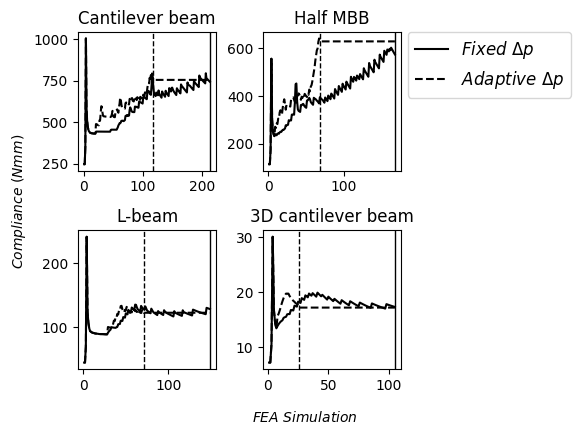
\includegraphics[width=\textwidth]{images/adaptive_csimp/convplots_csimp_03_01_80_001_ip.png}
    \caption{Convergence plots for CSIMP with and without penalty adaptation using $V = 0.3$, $tol = 0.01$, $\Delta p = 0.05$.}
    \label{fig:reuse_convplots_high_tol}
  \end{figure}
  \begin{figure}
    \centering
    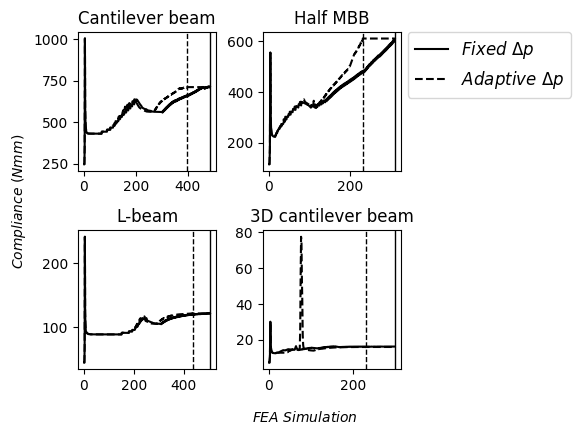
\includegraphics[width=\textwidth]{images/adaptive_csimp/convplots_csimp_03_0001_80_001_ip.png}
    \caption{Convergence plots for CSIMP with and without penalty adaptation using $V = 0.3$, $tol = 0.0001$, $\Delta p = 0.05$.}
    \label{fig:reuse_convplots_low_tol}
  \end{figure}

  Figures \ref{fig:reuse_convplots_high_tol} and \ref{fig:reuse_convplots_low_tol} show typical convergence plots for the test problems using high and low tolerances respectively with and without penalty adaptation. It is clear that the curves follow a similar pattern and converge to similar objective values but the penalty adaptation causes an acceleration to the convergence. In one case, the penalty adaptation curve had a higher peak which can be explained by the extreme changes in the objective of the current solution when skipping many subproblems optimization. 

  Overall, the results seem to suggest the need for a decreasing tolerance scheme to allow penalty adaptation to be more effective than when using a fixed low tolerance, while reaping the benefits of a low final tolerance in the objective value and reducing the \% frac of the continuous solution.

  \subsection{Decreasing tolerance}

  In the previous section, the effect of the tolerance on $\% frac$, C-Obj and D-Obj was observed. While a lower tolerance seems to have some undeniable benefits in most test problems, it is certainly more computationally expensive. It is therefore customary to use a decreasing tolerance scheme with $\theta < 1$ in Algorithm \ref{alg:cont_simp} since for low penalty values $p$ and low $\beta$, the solution is still highly fractional and therefore solving it to a low tolerance is thought to be unnecessary. Algorithm \ref{alg:cont_simp} uses an exponentially decaying tolerance curve. Other curves can also be used to raise the average tolerance of all the subproblems without changing the minimum and maximum tolerances. In this section, an exponentially decaying tolerance function will be used which starts at $tol_0$ in the first subproblem and ends at $tol_{min}$ in the last. For $tol_0 = 0.01$ and $tol_{min} = 0.0001$, using a $\Delta p_0 = 0.1$ corresponds to $\theta = 0.8913$, and using $\Delta p_0 = 0.05$ corresponds to $\theta = 0.9441$. Note that the tolerance is decreased in each subproblem and the new tolerance is used to decide whether the subproblem is worth solving or not as described in section \ref{sec:adaptive_penalty}. Given that penalty adaptation was observed to be more effective when using higher tolerances than lower ones, a decreasing tolerance scheme is likely to enhance the benefits of penalty adaptation. To avoid the skipping of all subproblems, the last subproblem will always be solved, i.e. never skipped. This should guarantee that the proposed algorithm has at least the same theoretical properties of a fixed penalty SIMP where $p = p_{max}$, thus making it theoretically no worse than the status quo. 

  \begin{table}[H]
\centering
\tabcolsep=0.09cm
% table caption is above the table
\caption{The problem type and parameter settings of the experiments with decreasing tolerance continuation SIMP. $tol_0 = 0.01$ and $tol_{min} = 1e-4$ were used in all test cases.}
\label{tab:exp_params2}
\begin{tabular}{|l|l|l|l||l|l|l|l|}
\hline\noalign{\smallskip}
Exp & Problem & $V$ & $\Delta p_0$ & Exp & Problem & $V$ & $\Delta p_0$ \\
\hline
1 & \multirow{ 4 }{*}{CantBeam} & \multirow{ 2 }{*}{0.3} & 0.1 & 9 & \multirow{ 4 }{*}{LBeam} & \multirow{ 2 }{*}{0.3} & 0.1 \\
2 & & & 0.05 & 10 & & & 0.05 \\
3 & & \multirow{ 2 }{*}{0.5} & 0.1 & 11 & & \multirow{ 2 }{*}{0.5} & 0.1 \\
4 & & & 0.05 & 12 & & & 0.05 \\
\hline
5 & \multirow{ 4 }{*}{HalfMBB} & \multirow{ 2 }{*}{0.3} & 0.1 & 13 & \multirow{ 4 }{*}{3D CantBeam} & \multirow{ 2 }{*}{0.3} & 0.1 \\
6 & & & 0.05 & 14 & & & 0.05 \\
7 & & \multirow{ 2 }{*}{0.5} & 0.1 & 15 & & \multirow{ 2 }{*}{0.5} & 0.1 \\
8 & & & 0.05 & 16 & & & 0.05 \\
\noalign{\smallskip}\hline
\end{tabular}
\end{table}

  \begin{table}
\centering
\tabcolsep=0.09cm
% table caption is above the table
\caption{This table shows the effect of penalty adaptation on CSIMP with decreasing tolerance. The table shows the results of the experiments studying the effect of solution reuse on: 1) the number of FEA simulations (Sims) required by CSIMP, 2) the final objective of the continuous NLP at $p = 5$ (C-Obj), 3) the objective value of the rounded discrete solution (D-Obj), and 4) the percentage of fractionness (\% frac). The parameters of each experiment are described in Table \ref{tab:exp_params2}.}
\label{tab:dec_tol_csimp_reuse}
\begin{tabular}{|l|l|l|l|l||l|l|}
\hline\noalign{\smallskip}
Exp & \multicolumn{3}{c||}{\textbf{Fixed $\Delta p = \Delta p_0$}} & \multicolumn{3}{c|}{\textbf{\% Increase due to $\Delta p$ adaptation}} \\
\noalign{\smallskip}\hline\noalign{\smallskip}
& \textbf{Sims} & \textbf{C-Obj / D-Obj} & \textbf{\% frac} & \textbf{Sims} & \textbf{C-Obj / D-Obj} & \textbf{\% frac}\\
\hline
1 & 185 & 814.2/581.6 & 17.3 & -14.6 & -8.8/-1.3 & -18.5 \\ 
\hline
2 &  316 & 720.4/553.1 & 14.0 & -16.5 & 4.1/6.2 & 0.7 \\ 
\hline
3 &  139 & 375.0/342.3 & 11.5 & -10.8 & -0.1/-0.0 & 0.0 \\ 
\hline
4 &  236 & 367.3/338.9 & 9.8 & -20.3 & 0.1/0.1 & 0.0 \\ 
\hline
\hline
5 & 130 & 619.6/293.9 & 24.6 & -25.4 & 0.4/-0.1 & 0.8 \\ 
\hline
6 & 260 & 606.5/292.8 & 24.3 & -39.6 & 2.6/-0.0 & 1.6 \\ 
\hline
7 & 130 & 219.5/175.3 & 18.1 & -26.2 & 0.2/0.7 & 0.6 \\ 
\hline
8 & 211 & 218.8/175.1 & 17.9 & -21.8 & -0.2/0.5 & -1.1 \\ 
\hline
\hline
9 & 153 & 121.5/103.4 & 9.0 & -20.3 & -0.1/0.6 & 0.0 \\ 
\hline
10 & 226 & 123.5/104.1 & 9.6 & -17.7 & 0.2/0.2 & 1.0 \\ 
\hline
11 & 142 & 69.8/65.6 & 6.8 & -31.7 & 0.1/0.2 & 0.0 \\ 
\hline
12 & 192 & 69.9/65.7 & 6.8 & -38.0 & 0.1/0.0 & 1.5 \\ 
\hline
\hline
13 & 97 & 16.1/13.1 & 10.1 & -41.2 & 0.0/0.0 & 1.0 \\ 
\hline
14 & 161 & 16.0/13.1 & 10.1 & -49.1 & 0.0/0.0 & 0.0 \\ 
\hline
15 & 97 & 10.2/9.3 & 10.9 & -39.2 & 0.0/0.0 & 0.0 \\ 
\hline
16 & 161 & 10.2/9.3 & 11.0 & -49.1 & 0.0/0.0 & 0.0 \\ 
\hline
\noalign{\smallskip}\hline
\end{tabular}
\end{table}


  \begin{figure}
    \centering
    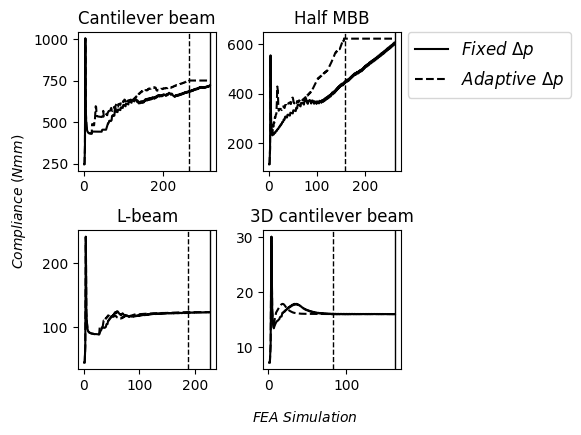
\includegraphics[width=\textwidth]{images/adaptive_csimp/convplots_dec_tol_csimp_03_0001_80_001_ip.png}
    \caption{Convergence plots of Dec-Tol CSIMP using $tol_0 = 0.01$, $tol_{min} = 0.0001$, $V = 0.3$, and $\Delta p = 0.05$ with and without penalty adaptation for the 4 test problems.}
    \label{fig:dec_tol_convplots}
  \end{figure}

  Figure \ref{fig:dec_tol_convplots} shows a typical convergence plot of the decreasing tolerance schemes with and without penalty step adaptation. It is clear that penalty adaptation was successful in many cases in accelerating the convergence of the algorithm for all the test problems, reducing the number of FEA simulations required by an average of 28.8 \%, without significant compromise to C-Obj, $4.1\%$ in the worst case. Finally, Figures \ref{fig:dec_tol_tops} and \ref{fig:dec_tol_tops2} show the final topologies of some of the test instances with and without penalty step adaptation using the decreasing tolerance scheme. For clarity, the binary solution is shown in the 3D case, while the continuous one is shown for the 2D problems.

  \begin{figure}
    \begin{subfigure}{0.45\textwidth}
      \centering
      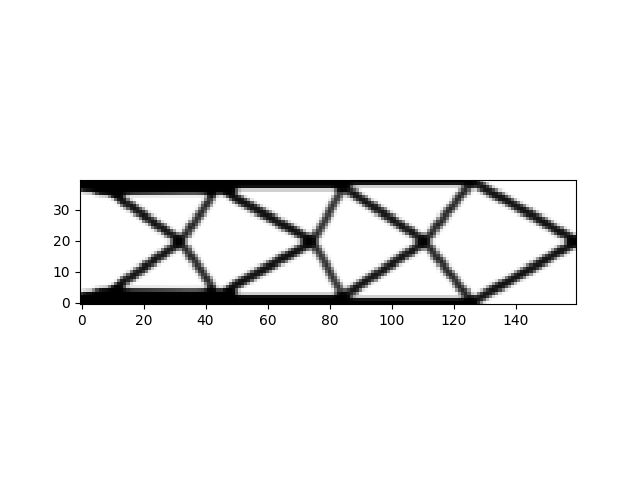
\includegraphics[width=1\textwidth]{images/adaptive_csimp/cantilever_dec_tol_csimp_03_0001_80_false_001_ip.png}
      \caption{Fixed $\Delta p = 0.05$, $V = 0.3$.}
    \end{subfigure} \hfill
    \begin{subfigure}{0.45\textwidth}
      \centering
      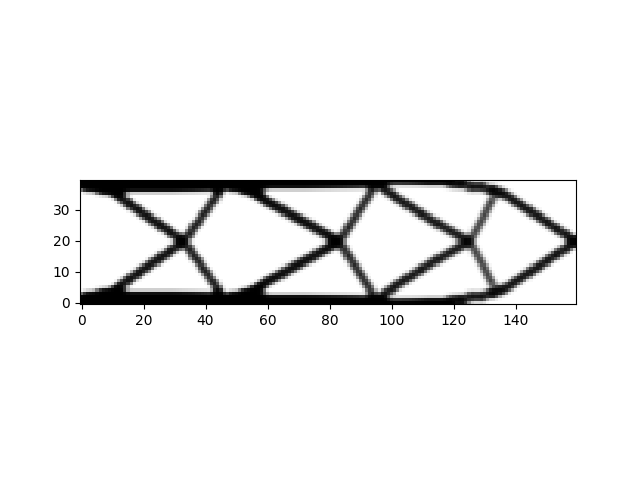
\includegraphics[width=1\textwidth]{images/adaptive_csimp/cantilever_dec_tol_csimp_03_0001_80_true_001_ip.png}
      \caption{Adaptive $\Delta p$, $\Delta p_0 = 0.05$, $V = 0.3$.}
    \end{subfigure}

    \begin{subfigure}{0.45\textwidth}
      \centering
      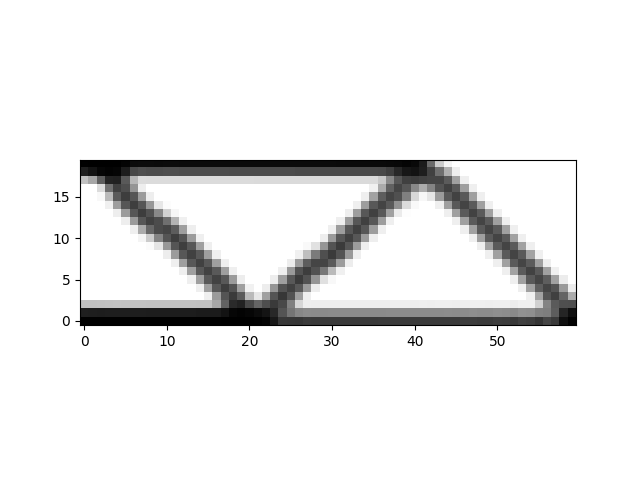
\includegraphics[width=1\textwidth]{images/adaptive_csimp/halfmbb_dec_tol_csimp_03_0001_80_false_001_ip.png}
      \caption{Fixed $\Delta p = 0.05$, $V = 0.3$.}
    \end{subfigure} \hfill
    \begin{subfigure}{0.45\textwidth}
      \centering
      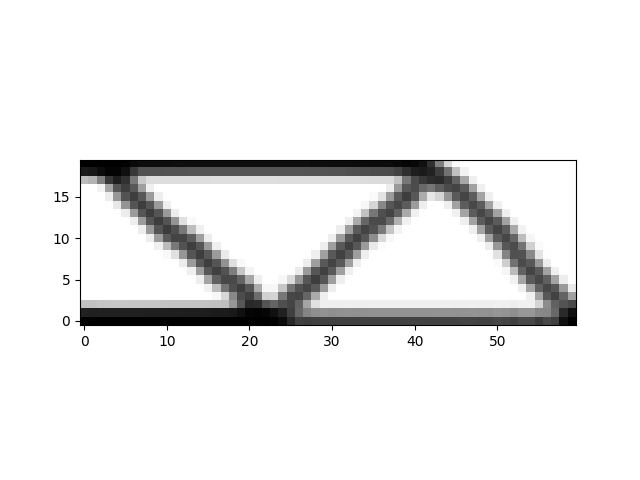
\includegraphics[width=1\textwidth]{images/adaptive_csimp/halfmbb_dec_tol_csimp_03_0001_80_true_001_ip.png}
      \caption{Adaptive $\Delta p$, $\Delta p_0 = 0.05$, $V = 0.3$.}
    \end{subfigure}

    \begin{subfigure}{0.45\textwidth}
      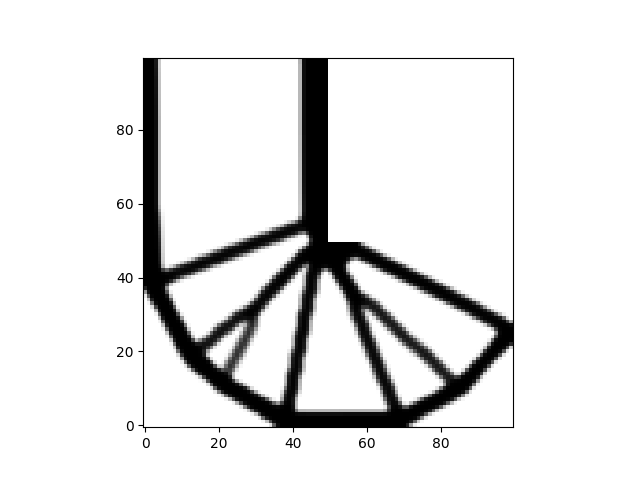
\includegraphics[width=1\textwidth]{images/adaptive_csimp/lbeam_dec_tol_csimp_03_0001_80_false_001_ip.png}
      \caption{Fixed $\Delta p = 0.05$, $V = 0.3$.}
    \end{subfigure} \hfill
    \begin{subfigure}{0.45\textwidth}
      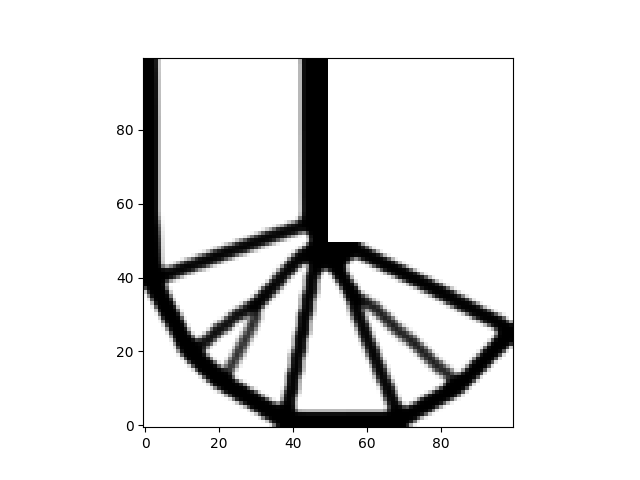
\includegraphics[width=1\textwidth]{images/adaptive_csimp/lbeam_dec_tol_csimp_03_0001_80_true_001_ip.png}
      \caption{Adaptive $\Delta p$, $\Delta p_0 = 0.05$, $V = 0.3$.}
    \end{subfigure}

    \caption{Continuous solutions of Dec-Tol CSIMP with a maximum tolerance of $0.01$ and a minimum tolerance of $0.0001$, with and without $\Delta p$ adaptation.}
    \label{fig:dec_tol_tops}
  \end{figure}

  \begin{figure}
    \begin{subfigure}{0.45\textwidth}
      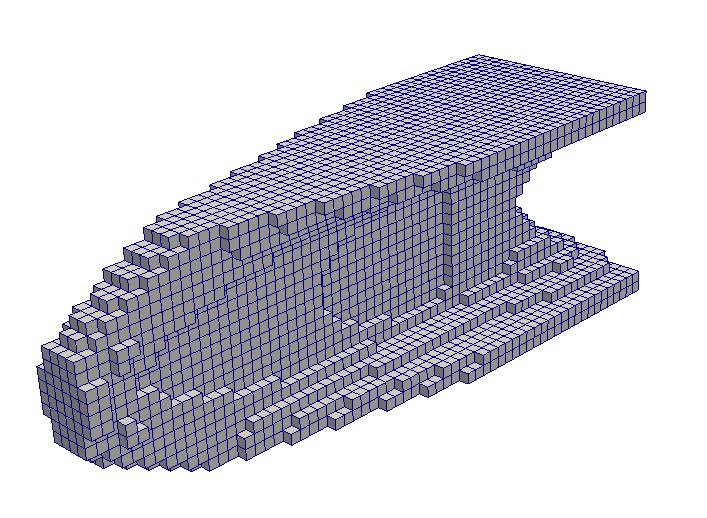
\includegraphics[width=1\textwidth]{images/adaptive_csimp/cantilever3d_false}
      \caption{Fixed $\Delta p = 0.05$, $V = 0.3$.}
    \end{subfigure} \hfill
    \begin{subfigure}{0.45\textwidth}
      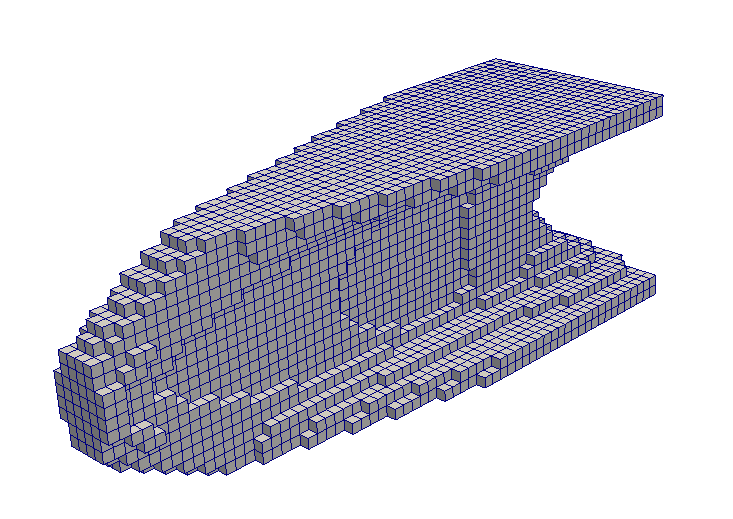
\includegraphics[width=1\textwidth]{images/adaptive_csimp/cantilever3d_true}
      \caption{Adaptive $\Delta p$, $\Delta p_0 = 0.05$, $V = 0.3$.}
    \end{subfigure}

    \caption{Binary solutions of the 3D cantilever beam problem using Dec-Tol CSIMP with a maximum tolerance of $0.01$ and a minimum tolerance of $0.0001$, with and without $\Delta p$ adaptation.}
    \label{fig:dec_tol_tops2}
  \end{figure}

  % Intermediate

  To further highlight that the reduction in the number of FEA simulations due to penalty adaptation is not trivial, Figure \ref{fig:intermediate_solution_lbeam} shows the intermediate solution of Dec-Tol CSIMP without penalty adaptation when solving the L-beam problem in Exp 10, $V = 0.3$, and $\Delta p = 0.05$ after 186 FEA simulations. Dec-Tol CSIMP with penalty adaptation only required 186 FEA simulations to converge for this problem while Dec-Tol CSIMP without penalty adaptation required 226. The intermediate solution, shown in Figure \ref{fig:cont_intermediate_solution_lbeam} is infeasible due to disconnected parts. The compliance of the binary solution is therefore not defined. This is in contrast to Figure \ref{fig:solution_final_lbeam_csimp_true} which shows the solution when using penalty adaptation after the same number of FEA simulations as Figure \ref{fig:intermediate_solution_lbeam}.

  \begin{figure}
    \centering
    \begin{subfigure}[t]{0.45\textwidth}
      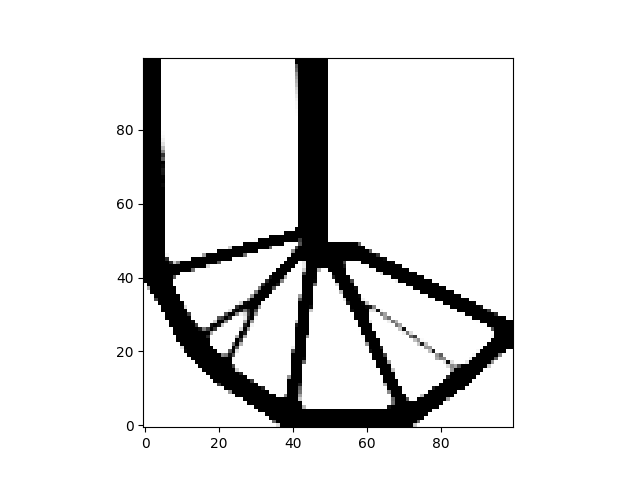
\includegraphics[width=0.9\textwidth]{images/adaptive_csimp/lbeam_dec_tol_csimp_intermediate_03_001_80.png}
      \caption{Continuous intermediate solution.}
      \label{fig:cont_intermediate_solution_lbeam}
    \end{subfigure} \hfill
    \begin{subfigure}[t]{0.45\textwidth}
      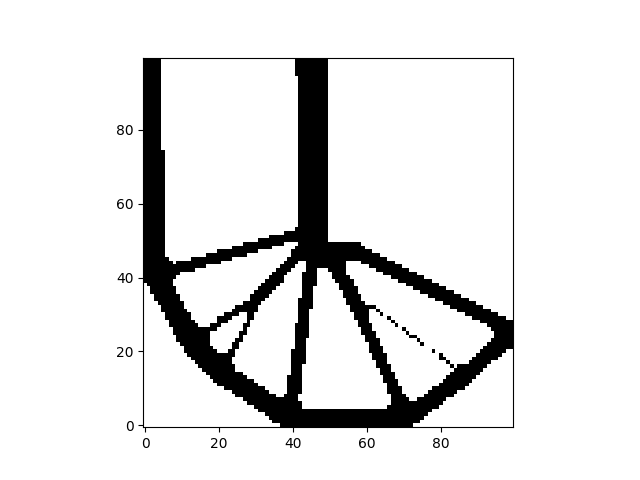
\includegraphics[width=0.9\textwidth]{images/adaptive_csimp/lbeam_dec_tol_csimp_intermediate_binary_03_001_80.png}
      \caption{Projected binary intermediate solution.}
      \label{fig:bin_intermediate_solution_lbeam}
    \end{subfigure}
    \caption{The continuous and projected intermediate solutions of the L-beam problem using Dec-Tol CSIMP without penalty adaptation after 186 FEA simulations using $V = 0.3$, and $\Delta p = 0.05$. CSIMP with penalty adaptation requires only 186 FEA simulations to converge, whereas without penalty adaptation, it takes 226 FEA simulations.}
    \label{fig:intermediate_solution_lbeam}
  \end{figure}

  \begin{figure}
    \centering
    \begin{subfigure}[t]{0.45\textwidth}
      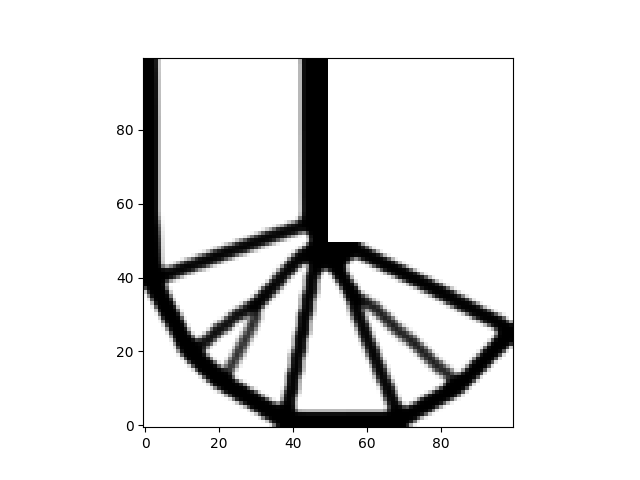
\includegraphics[width=0.9\textwidth]{images/adaptive_csimp/lbeam_dec_tol_csimp_03_0001_80_true_001_ip.png}
      \caption{This is the final continuous solution. The objective value is 123.7.}
      \label{fig:solution_final_lbeam_cont_csimp_true}
    \end{subfigure} \hfill
    \begin{subfigure}[t]{0.45\textwidth}
      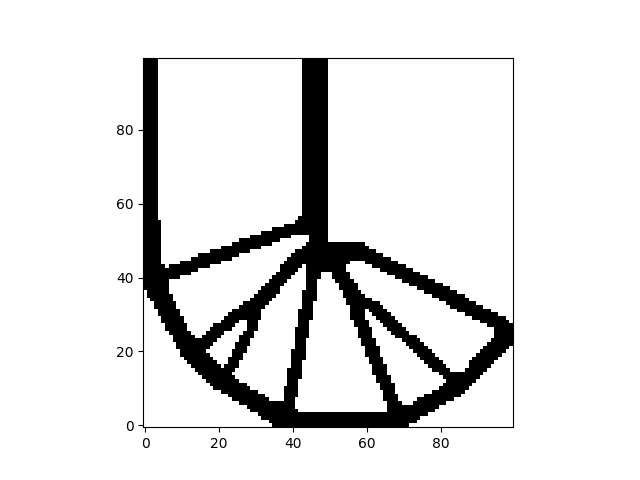
\includegraphics[width=0.9\textwidth]{images/adaptive_csimp/lbeam_dec_tol_csimp_binary_03_0001_80_true.png}
      \caption{This is the projected final solution where $x_e$ is binary for all $e$. The objective value is 104.3.}
      \label{fig:solution_final_lbeam_binary_csimp_true}
    \end{subfigure}
    \caption{The continuous and projected final solutions of the L-beam problem using Dec-Tol CSIMP with penalty adaptation using $V = 0.3$, and $\Delta p = 0.05$. Convergence happened after 186 FEA simulations.}
    \label{fig:solution_final_lbeam_csimp_true}
  \end{figure}

\section{Effect of $x_{min}$} \label{sec:xmin_sens}

  In the vast majority of papers in literature, the value of $x_{min}$ used is 0.001. Some papers seem to penalize the value of $0 \leq x_e \leq 1$ while others seem to penalize the value of $\rho_e = x_e (1 - x_{xmin}) + x_{min}$. In this chapter, the former has been used. The latter has the effect of decreasing the minimum value that $\rho_e$ can take as the penalty increases. While the mentioned reason for using $x_{min} > 0$ in literature is to stop the stiffness matrix $\bm{K}$ from becoming singular, this is not free of limitations. In this section, it will be proven that in the VCCM problem, $x_{min}$ plays the role of a penalty for 2 types of infeasible designs: 1) a design with a force on a node with no element to support it, and 2) a design with rigid body modes on which a non-orthogonal force is applied, i.e. the force has a component along one or more of the rigid body modes. The effect of $x_{min}$ on the number of FEA simulations required to solve the problem will then be presented.

  Let the nodes that have all their elements removed, i.e. $x_e = 0$, be called \textit{shadow nodes}, and let any degree of freedom (dof) of a shadow node be called a \textit{shadow dof}. In the case where $x_{min} = 0$, shadow dofs do not have any non-zero value in their corresponding rows and columns of the stiffness matrix $\bm{K}$. A low $x_{min}$ approximates this without letting $\bm{K}$ become singular. Experiments show that the nodal displacements and compliance of the optimal solutions often reach a finite limit value as $x_{min} \to 0$ for the optimal topologies, with non-zero displacements for the shadow nodes. When $x_{min}$ is 0, $\bm{K}$ becomes rank deficient if a shadow dof exists. Note that: 
  \begin{align}
    \bm{u} = \bm{K}^{-1} \bm{f} = \sum_j \frac{1}{\lambda_j} \bm{v}_j \bm{v}_j^T \bm{f}
  \end{align}
  where $\bm{v}_j$ is the $j^{th}$ eigenvector of $\bm{K}$ and $\lambda_j$ is the corresponding eigenvalue. Additionally, without loss of generality, let the $i^{th}$ dof be a shadow dof that has no Dirichlet boundary condition. It is easy to show that as $x_{min}$ goes to 0, that the span of the eigenspace of $\bm{K}$ associated with the eigenvalue of 0, admits a new basis vector $\bm{e}_i$, where $\bm{e}_i$ is the $i^{th}$ standard basis vector. This is easy to see since the matrix $\bm{K}$'s $i^{th}$ row and column are all zeros, so $\bm{K} \bm{e}_i = 0 \times \bm{e}_i$. Given the limit eigenvector, $\bm{e}_i$, one can also obtain the limit eigenvalue using the Rayleigh quotient $\frac{\bm{e}^T_i \bm{K} \bm{e}_i}{\bm{e}^T_i \bm{e}_i} = K_{ii} = x_{min} \times \sum_e K_{e,ii}$, where $K_{ii}$ is the $i^{th}$ diagonal element of the matrix $\bm{K}$, $\bm{K}_e$ is the extended form of the element stiffness matrix of the element $e$ such that $\bm{K}_e$ is the same size as $\bm{K}$ but only has non-zeros where element $e$'s degrees of freedom are, and $K_{e,ii}$ is $i^{th}$ diagonal element of $\bm{K}_e$. The following relationship therefore holds:
  \begin{align}
    \lim_{x_{min} \to 0} \bm{u} & = \lim_{x_{min} \to 0} \sum_j \frac{1}{\lambda_j} \bm{v}_j \bm{v}_j^T \bm{f} \\ 
    & = \lim_{x_{min} \to 0} \frac{1}{\lambda_i} \bm{v}_i \bm{v}_i^T \bm{f} + \sum_{j \neq i} \frac{1}{\lambda_j} \bm{v}_j \bm{v}_j^T \bm{f} \\
    & = \lim_{x_{min} \to 0} \frac{1}{x_{min} \times \sum_e K_{e,ii}} \bm{e}_i \bm{e}_i^T \bm{f} + \sum_{j \neq i} \frac{1}{\lambda_j} \bm{v}_j \bm{v}_j^T \bm{f}\\
    & = \lim_{x_{min} \to 0} \frac{f_i}{x_{min} \times \sum_e K_{e,ii}} \bm{e}_i + \sum_{j \neq i} \frac{1}{\lambda_j} \bm{v}_j \bm{v}_j^T \bm{f}
  \end{align}
  where $f_i$ is the $i^{th}$ element of the vector $\bm{f}$. Notice that if $f_i = 0$, the limit of the first term will be 0. Whereas, if $f_i \neq 0$, the limit will be $\pm \infty$ depending on the sign of $f_i$. The above derivations give a natural necessary condition for the finiteness of the displacements $\bm{u}$ and the compliance $C$. If the displacements and hence the compliance are to be finite, all shadow degrees of freedom should have no force component corresponding to them. In other words, every force should have at least one element to support it.

  The above condition can be enforced with constraints or it can be enforced by making $x_{min}$ small enough. Let $x_{min}$ be small enough, so we can approximate $\bm{u}$ by its limit term:
  \begin{align}
    \bm{u} & \approx \sum_{i \in I} \frac{f_i}{x_{min} \times \sum_e K_{e,ii}} \bm{e}_i + \sum_{j \notin I} \frac{1}{\lambda_j} \bm{v}_j \bm{v}_j^T \bm{f}
  \end{align}
  where $I$ is the set of shadow dofs. The compliance $C = \bm{f}^T \bm{u}$ can therefore be approximated by:
  \begin{align}
    C & \approx \sum_{i \in I} \frac{f^2_i}{x_{min} \times \sum_e K_{e,ii}} + \sum_{j \notin I} \frac{1}{\lambda_j} (\bm{v}_j^T \bm{f})^2
  \end{align}

  Since $\bm{K}$ is positive semi-definite, $\lambda_j \geq 0 \quad \forall j$. So we can approximately lower bound the compliance $C$ using:
  \begin{align}
    C \gtrapprox \sum_{i \in I} \frac{f^2_i}{x_{min} \times \sum_e K_{e,ii}}
  \end{align}

  Therefore, one can see that a lower $x_{min}$ \textit{penalizes} the compliance of the designs with shadow degrees of freedom corresponding to a force component. This means that if the binary solution projected from the optimal continuous one introduces shadow dofs, then the value of $x_{min}$ may not have been small enough. In other words, a higher $x_{min}$ increases the chances of getting an \textit{optimal} design with a shadow dof where a force component is applied. This is clearly not a feasible design in the exact sense. The above derivations also suggest the possibility of using a weighted compliance term in the objective in classes of topology optimization problems other than VCCM to trigger the penalization effect of $x_{min}$.

  Similar derivations can be followed to show that $x_{min}$ also penalizes a design with rigid body modes. Let $\bm{K}(x_{min})$ be the stiffness matrix of a disconnected binary design for some value of $x_{min}$. Since $\bm{K}$ is positive definite when $x_{min} > 0$, $\bm{u}^T \bm{K} \bm{u} > 0 \quad \forall \bm{u}$. Let $\bm{v}_i$ be the $i^{th}$ rigid body mode of a subset of the elements, e.g. a disconnected piece, when $x_{min} = 0$. Since $\bm{v}_i$ is a rigid body mode, $\bm{v}_i^T \bm{K}(0) \bm{v}_i = 0$. Let $\bm{K} = \bm{K}_{f_i} + \bm{K}_{p_i} + x_{min} \times \bm{K}_{v_i}$ be the decomposition of $\bm{K}$ into free, pinned and void components of the binary design, respectively, with respect to the rigid body mode $\bm{v}_i$. $\bm{K}_{f_i}$ is assembled from the solid elements that the rigid body mode $\bm{v}_i$ moves, $\bm{K}_{p_i}$ is assembled from the remaining solid elements, and $\bm{K}_{v_i}$ is assembled from the void elements. Let $\bm{K}$ have the boundary conditions properly applied, with the Dirichlet dofs having only a positive diagonal term in $\bm{K}$. If such a dof is part of 2 matrices of $\bm{K}_{f_i}$, $\bm{K}_{p_i}$ and $\bm{K}_{v_i}$, half the value can be used in each. Let's first consider the case where the component with the free body mode is disconnected from the pinned component. Since $\bm{v}_i$ is a rigid body mode of the elements making up $\bm{K}_{f_i}$, and the set of dofs of $\bm{K}_{p_i}$ is disjoint from the set of dofs making up $\bm{K}_{f_i}$, $\bm{v}_i^T \bm{K}_{f_i} \bm{v}_i = \bm{v}_i^T \bm{K}_{p_i} \bm{v}_i = 0$. The same holds for the case where the free component is not fully disconnected but hinged on a point, or a line in 3D space, since the dofs of the hinge do not contribute to the rigid body mode. Therefore, $\bm{v}_i^T \bm{K} \bm{v}_i = x_{min} \times \bm{v}_i^T \bm{K}_{v_i} \bm{v}_i$. Assuming $\bm{v}_i$ is a unit vector, $\bm{v}_i^T \bm{K} \bm{v}_i$ is the Rayleigh quotient of the limit eigenvector $\bm{v}_i$ corresponding to a 0 eigenvalue, as $x_{min} \to 0$. Therefore, the following holds:
  \begin{align}
    \lim_{x_{min} \to 0} \bm{u} & = \lim_{x_{min} \to 0} \bm{K}(x_{min})^{-1} \bm{f}\\
    & = \lim_{x_{min} \to 0} \sum_{i \in J} \frac{\bm{v}_i^T \bm{f}}{x_{min} \times \bm{v}_i^T \bm{K}_{v_i} \bm{v}_i} \bm{v}_i + \sum_{j \notin J} \frac{1}{\lambda_j} \bm{v}_j \bm{v}_j^T \bm{f}
  \end{align}
  where $\{\bm{v}_i: i \in J\}$ is the set of rigid body modes at $x_{min} = 0$. Note that the second term above can further be broken down into 2 terms, one for the shadow dofs, and one for the remaining components:
  \begin{align}
    \lim_{x_{min} \to 0} \bm{u} & = \lim_{x_{min} \to 0} \sum_{i \in I} \frac{f_i}{x_{min} \times \sum_e K_{e,ii}} \bm{e}_i + \sum_{i \in J} \frac{\bm{v}_i^T \bm{f}}{x_{min} \times \bm{v}_i^T \bm{K}_{v_i} \bm{v}_i} \bm{v}_i + \sum_{j \notin I, j \notin J} \frac{1}{\lambda_j} \bm{v}_j \bm{v}_j^T \bm{f}
  \end{align}

  The limit compliance can then be written as:
  \begin{align}
    \lim_{x_{min} \to 0} C & = \lim_{x_{min} \to 0} \sum_{i \in I} \frac{f_i^2}{x_{min} \times \sum_e K_{e,ii}} + \sum_{i \in J} \frac{(\bm{v}_i^T \bm{f})^2}{x_{min} \times \bm{v}_i^T \bm{K}_{v_i} \bm{v}_i} + \sum_{j \notin I} \frac{(\bm{v}_j^T \bm{f})^2}{\lambda_j}
  \end{align}

  When $x_{min}$ is small enough that one can use the limit expression to approximate the value of $C$, one can see that $x_{min}$ indeed plays the role of a penalty for any design with a shadow dof $i$ and a force component $f_i \neq 0$, or any design with a rigid body mode on which a non-orthogonal force is applied such that $\bm{v}_i^T \bm{f} \neq 0$.
  \begin{align}
    C \gtrapprox \sum_{i \in I} \frac{f^2_i}{x_{min} \times \sum_e K_{e,ii}} + \sum_{i \in J} \frac{(\bm{v}_i^T \bm{f})^2}{x_{min} \times \bm{v}_i^T \bm{K}_v \bm{v}_i}
  \end{align}

  The experimental results shown in Table \ref{tab:dec_tol_csimp_xmin} indicate that a higher value of $x_{min}$ can lead to faster convergence. This is not surprising since MMA uses first order approximation of the objective and constraints. So if the objective function varies significantly in the neighbourhood of local minima, the first order approximation is likely to cause the solution to jump from one basin of attraction to another during an MMA iteration. However, too high a value can lead to a final design that is infeasible in the exact sense. From the above approximate lower bound expression, one can see that the best choice of $x_{min}$ is very much problem-dependent. This is because the penalization effect of $x_{min}$ is undermined if the norm of $\bm{K}_e$ is increased for all $e$. One way to increase the norm of $\bm{K}_e$ is to use a higher Young's modulus $E$.

  A better way to choose the value of $x_{min}$ is to make sure that $x_{min} = \frac{\epsilon}{\lambda_{max}}$, where $\epsilon$ is a small number and $\lambda_{max}$ is the maximum eigenvalue of the stiffness matrix of the ground mesh. It is simple to show that $\sum_e K_{e,ii}$ and $\bm{v}_i^T \bm{K}_{v_i} \bm{v}_i$ are both less than or equal to $\lambda_{max}$. 

  \begin{proof}
    Let $\lambda_{min}$ and $\lambda_{max}$ be the minimum and maximum eigenvalues of the positive definite matrix $\bm{K}$ at the ground mesh, respectively. It is well known that:
    \begin{align}
      &  0 < \lambda_{min} \leq \frac{\bm{x}^T \bm{K} \bm{x}}{\bm{x}^T \bm{x}} \leq \lambda_{max} \quad \forall \bm{x} \in \mathbb{R}^n
    \end{align}
    where $n$ is the number of degrees of freedom \cite{Golub1996}. This inequality holds for all $\bm{x} \in \mathbb{R}^n$ including the standard basis vector $\bm{e}_i$ corresponding to the $i^{th}$ shadow dof as well as any orthonormal rigid body mode $\bm{v}_i$.
    \begin{align}
      &  0 < \lambda_{min} \leq \bm{e}_i^T \bm{K} \bm{e}_i = \sum_e K_{e,ii} \leq \lambda_{max} \\
      &  0 < \lambda_{min} \leq \bm{v}_i^T \bm{K} \bm{v}_i \leq \lambda_{max}
    \end{align}
    Additionally, since each element stiffness matrix $\bm{K}_e$ is positive semi-definite, $\bm{K}_{f_i}$, $\bm{K}_{p_i}$ and $\bm{K}_{v_i}$ are all positive semi-definite with a non-negative quadratic form. Therefore:
    \begin{align}
      & \bm{v}_i^T \bm{K}_{v_i} \bm{v}_i \leq \bm{v}_i^T \bm{K}_{f_i} \bm{v}_i + \bm{v}_i^T \bm{K}_{p_i} \bm{v}_i + \bm{v}_i^T \bm{K}_{v_i} \bm{v}_i = \bm{v}_i^T \bm{K} \bm{v}_i \leq \lambda_{max}
    \end{align}
    \textit{This completes the proof}.
  \end{proof}

  Let $LB = \sum_{i \in I} \frac{f^2_i}{x_{min} \times \sum_e K_{e,ii}} + \sum_{i \in J} \frac{(\bm{v}_i^T \bm{f})^2}{x_{min} \times \bm{v}_i^T \bm{K}_{v_i} \bm{v}_i}$. If $x_{min} = \frac{\epsilon}{\lambda_{max}}$:
  \begin{align}
    LB & \geq \sum_{i \in I} \frac{f^2_i}{\epsilon} + \sum_{i \in J} \frac{(\bm{v}_i^T \bm{f})^2}{\epsilon} \\
    C & \gtrapprox \frac{1}{\epsilon} \Bigg( \sum_{i \in I} f^2_i + \sum_{i \in J} (\bm{v}_i^T \bm{f})^2 \Bigg)
  \end{align} 
  Therefore, penalization will not be undermined by the scale of $\bm{K}$. Choosing an appropriate value of $\epsilon$ is not an easy task. It needs to be small enough so that designs in the neighbourhood with one of the 2 penalized cases have a worse compliance than other feasible designs, in the exact sense of feasibility. A future research direction can be on efficient ways to choose and adapt the value of $\epsilon$. Figure \ref{fig:high_xmin_solution_cantilever} shows the final continuous design of Dec-Tol CSIMP without penalty adaptation using $x_{min} = 0.01$ and $x_{min} = 0.001$, for volume fraction $V = 0.1$. It is clear that the second infeasibility case is present. Note that unlike $x_{min}$, $\epsilon$ is not a dimensionless quantity. $\epsilon$ has the same unit as the elements of the stiffness matrix, i.e. $N/mm$.

  \begin{table}
\centering
\tabcolsep=0.09cm
% table caption is above the table
\caption{This table shows the effect of increasing $x_{min}$ on CSIMP with decreasing tolerance and a fixed penalty step. The table shows the results of the experiments studying the effect of increasing $x_{min}$: 1) the number of FEA simulations (Sims) required by CSIMP, 2) the final objective of the continuous NLP at $p = 5$ (C-Obj), 3) the objective value of the rounded discrete solution (D-Obj), and 4) the percentage of fractionness (\% frac). The parameters of each experiment are described in Table \ref{tab:exp_params2}.}
\label{tab:dec_tol_csimp_xmin}
\begin{tabular}{|l|l|l|l|l||l|l|}
\hline\noalign{\smallskip}
Exp & \multicolumn{3}{c||}{\textbf{$x_{min} = 0.001$}} & \multicolumn{3}{c|}{\textbf{\% Increase - $x_{min} = 0.01$}} \\
\noalign{\smallskip}\hline\noalign{\smallskip}
& \textbf{Sims} & \textbf{C-Obj / D-Obj} & \textbf{\% frac} & \textbf{Sims} & \textbf{C-Obj / D-Obj} & \textbf{\% frac}\\
\hline
1 & 185 & 814.2/581.6 & 17.3 & -23.8 & -16.4/-4.2 & -18.5 \\ 
\hline
2 &  316 & 720.4/553.1 & 14.0 & -29.7 & -5.9/2.8 & 0.0 \\ 
\hline
3 &  139 & 375.0/342.3 & 11.5 & -15.1 & -3.3/-1.3 & -12.2 \\ 
\hline
4 &  236 & 367.3/338.9 & 9.8 & -23.3 & -1.5/-0.1 & 2.0 \\ 
\hline
\hline
5 & 130 & 619.6/293.9 & 24.6 & -7.7 & -13.9/14.0 & -0.8 \\ 
\hline
6 & 260 & 606.5/292.8 & 24.3 & -21.2 & -12.4/9.6 & 0.0 \\ 
\hline
7 & 130 & 219.5/175.3 & 18.1 & -7.7 & -2.9/1.0 & -0.6 \\ 
\hline
8 & 211 & 218.8/175.1 & 17.9 & -6.6 & -2.6/1.1 & 1.1 \\ 
\hline
\hline
9 & 153 & 121.5/103.4 & 9.0 & -20.9 & -3.0/1.3 & 1.1 \\ 
\hline
10 & 226 & 123.5/104.1 & 9.6 & -14.6 & -4.7/0.5 & -5.2 \\ 
\hline
11 & 142 & 69.8/65.6 & 6.8 & -26.8 & -0.9/0.5 & -4.4 \\ 
\hline
12 & 192 & 69.9/65.7 & 6.8 & -12.0 & -1.1/0.2 & -2.9 \\ 
\hline
\hline
13 & 97 & 16.1/13.1 & 10.1 & -1.0 & -1.9/0.0 & 2.0 \\ 
\hline
14 & 161 & 16.0/13.1 & 10.1 & 0.0 & -1.2/0.0 & 1.0 \\ 
\hline
15 & 97 & 10.2/9.3 & 10.9 & 0.0 & -1.0/0.0 & -0.9 \\ 
\hline
16 & 161 & 10.2/9.3 & 11.0 & 0.0 & -1.0/0.0 & -0.9 \\ 
\hline
\noalign{\smallskip}\hline
\end{tabular}
\end{table}


  \begin{figure}[H]
    \centering
    \begin{subfigure}{0.45\textwidth}
      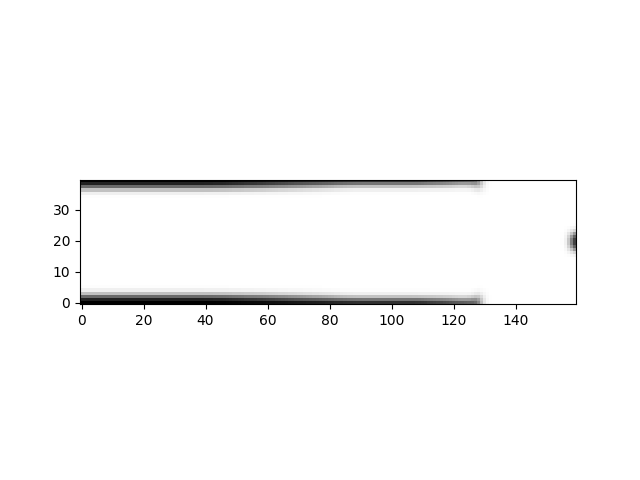
\includegraphics[width=0.9\textwidth]{./images/adaptive_csimp/cantilever_dec_tol_csimp_01_0001_80_false_01_ip.png}
      \caption{$x_{min} = 0.01$.}
    \end{subfigure} \hfill
    \begin{subfigure}{0.45\textwidth}
      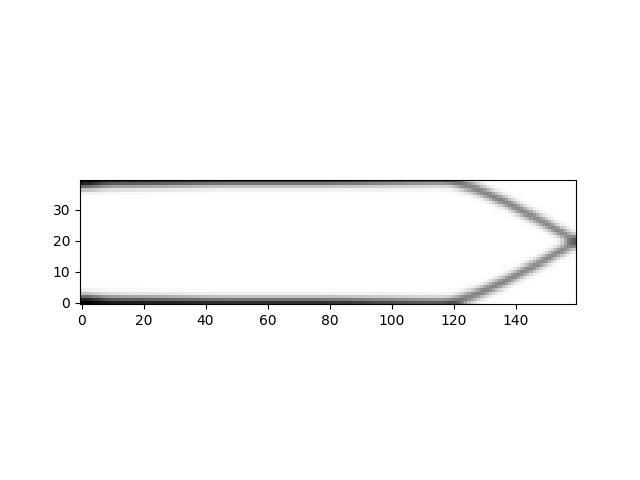
\includegraphics[width=0.9\textwidth]{./images/adaptive_csimp/cantilever_dec_tol_csimp_01_0001_80_false_001_ip.png}
      \caption{$x_{min} = 0.001$.}
    \end{subfigure}
    \caption{2D cantilever problem using Dec-Tol CSIMP without penalty adaptation using $V = 0.1$, $\Delta p = 0.05$.}
    \label{fig:high_xmin_solution_cantilever}
  \end{figure}

\section{Conclusion} \label{sec:conclusion}

  In this chapter, a penalty step adaptation technique for the continuation SIMP algorithm was proposed and tested. Four common test problems from literature, three 2D and one 3D, were used to test the efficacy of the penalty adaptation with different parameter settings. The main factors affecting the efficacy of the penalty adaptation in the CSIMP algorithm in reducing the number of FEA simulations needed to converge to the final solution were identified. The experimental results demonstrate a significant reduction in the number of FEA simulations required to reach the optimal solution in the decreasing tolerance continuation SIMP algorithm, with exponentially decaying tolerance, with little to no detriment in the objective value and the other metrics used. Finally, a mathematical and experimental treatment of the effect of $x_{min}$ on the convergence of the SIMP algorithm was given with some recommendations for choosing a suitable $x_{min}$.


\clearpage
\newpage
